\documentclass[a4paper, 11pt]{article}

\usepackage[utf8]{inputenc}
\usepackage[T1]{fontenc}

\usepackage[french,noconfigs]{babel}
\usepackage{lmodern}

\usepackage{graphicx}

\begin{document}

  \section{Format}

    Choisissez bien le format de vos images. En général n'importe quel format de base passe. Mais quand vous compilez en \verb!.ps! vous ne pouvez utiliser que des images postscript (\verb!.eps!).

    En général, préférez le format \verb!.pdf! pour les images vectorielles, et le format \verb!.jpg! pour les autres. Avec \emph{GIMP} vous pouvez faire à peu près toutes les conversions nécessaires.

    \section{Insérer une image}

    On utilise le package \fbox{\verb!graphicx!} pour insérer des images.

    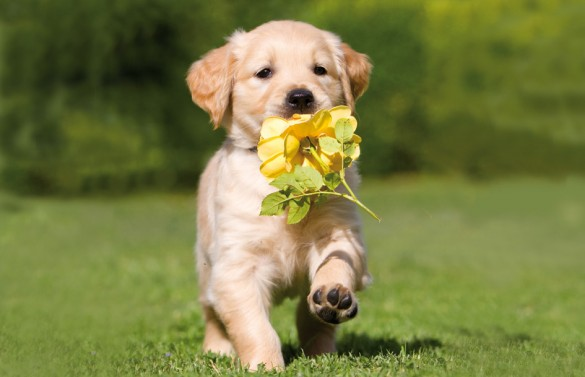
\includegraphics[width=3cm]{img/chien.jpg}
    \shortstack{1cm \\ \rule{1cm}{1cm}}
    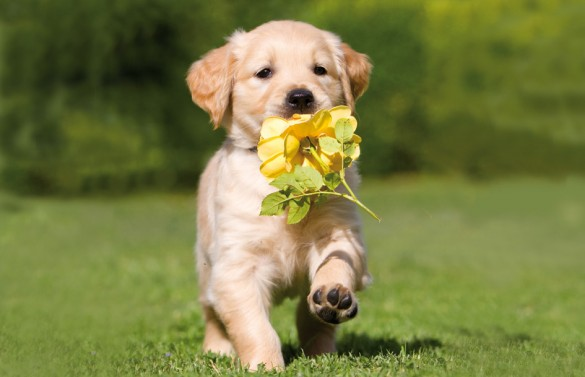
\includegraphics[height=5cm]{img/chien.jpg}

    \noindent 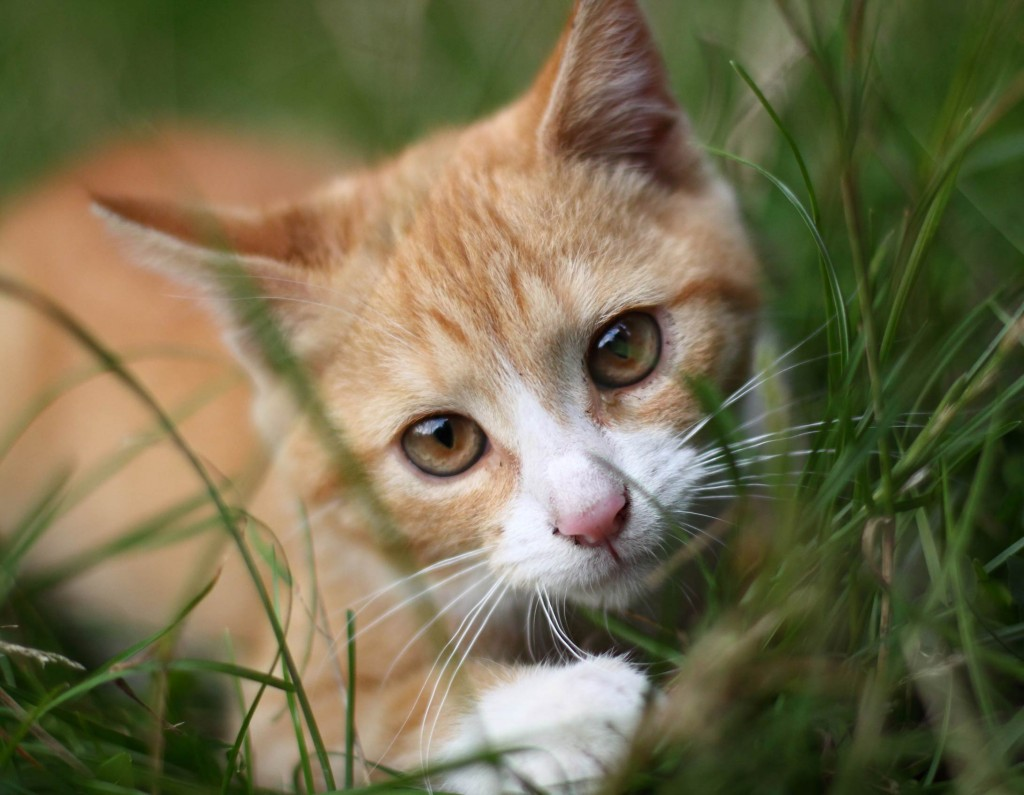
\includegraphics[width=6cm,height=2cm]{img/chat.jpg}
    \shortstack{1cm \\ \rule{1cm}{1cm}}
    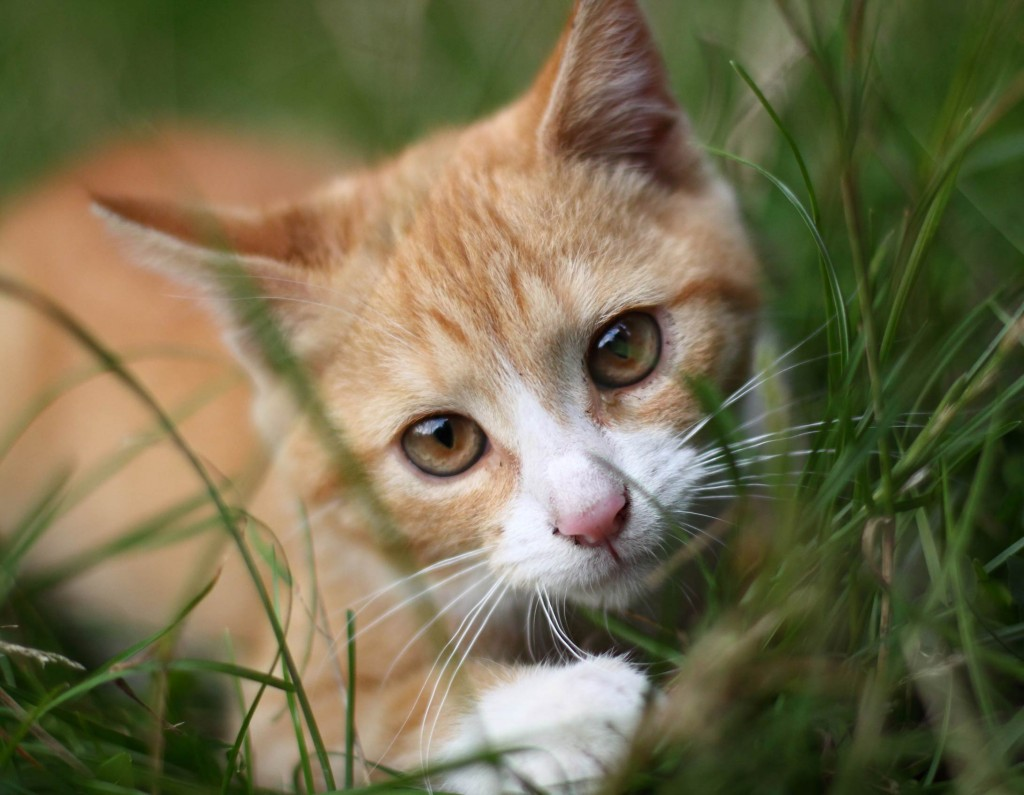
\includegraphics[width=6cm,height=2cm,keepaspectratio]{img/chat.jpg}
    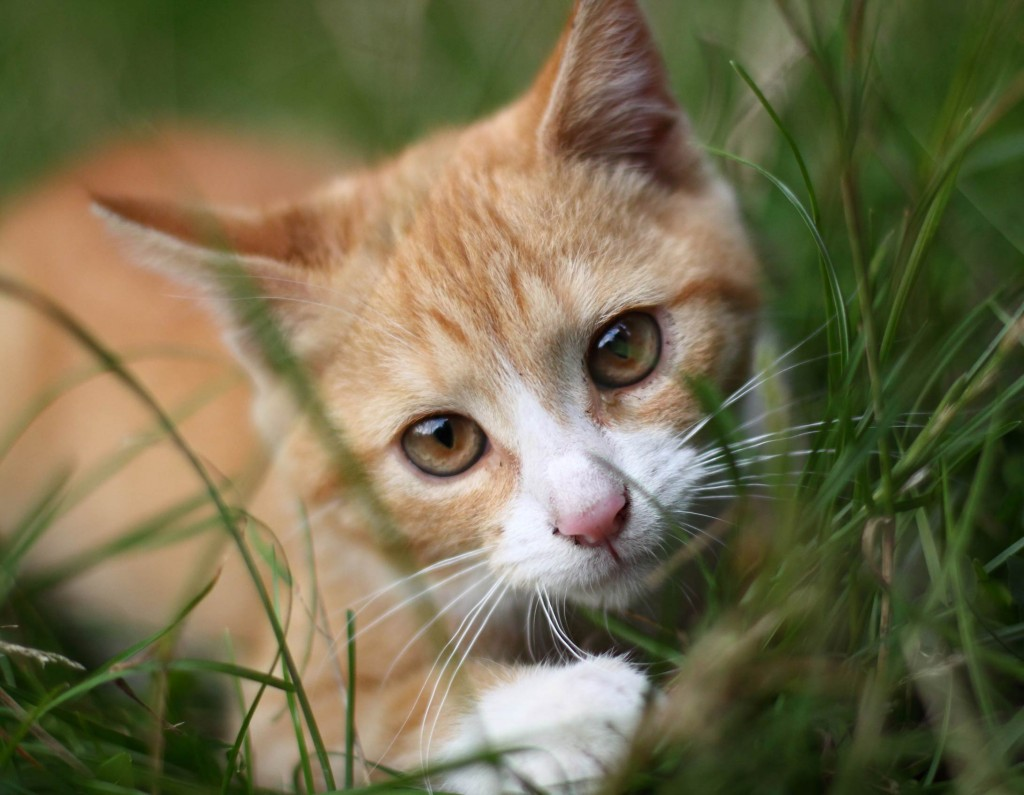
\includegraphics[scale=0.1]{img/chat.jpg}

    \noindent 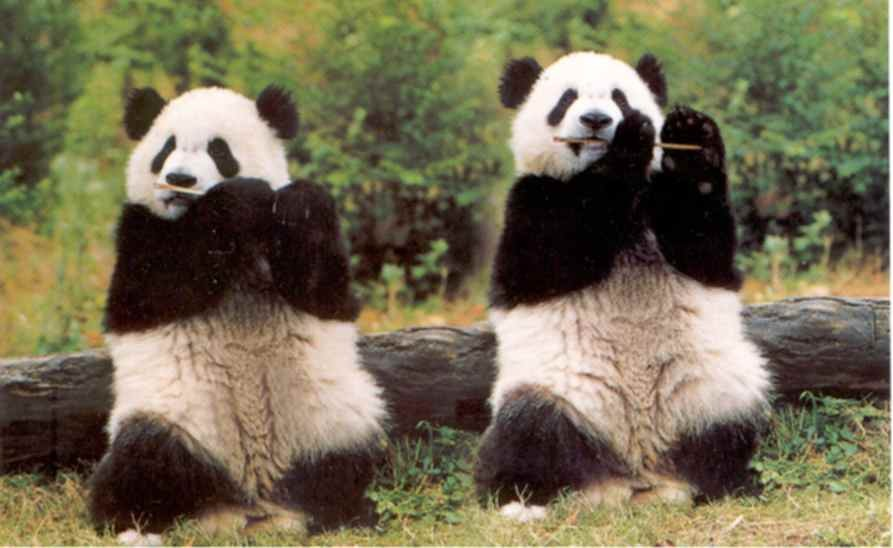
\includegraphics[height=4cm]{img/panda.jpg}
    \shortstack{1cm \\ \rule{1cm}{1cm}}
    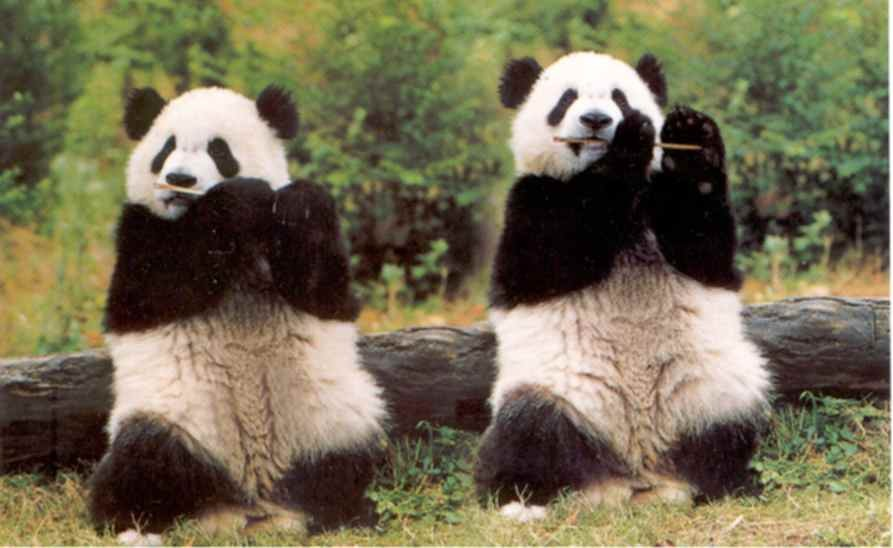
\includegraphics[height=4cm,clip,trim=1cm 0cm 8cm 1cm]{img/panda.jpg} % trim = g b d h

    \begin{figure}[h]
        \centering
        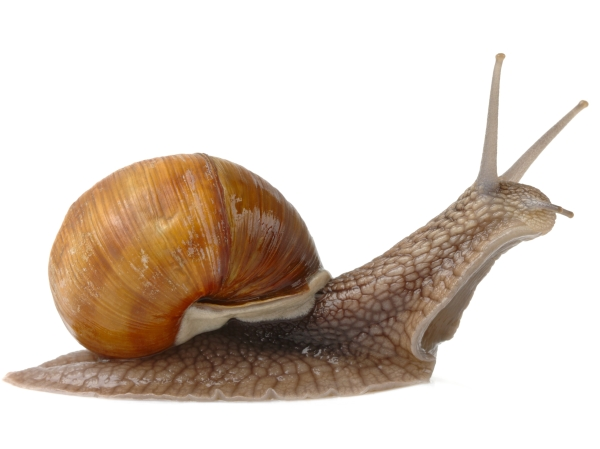
\includegraphics[width=0.7\textwidth,angle=45]{img/escargot.jpg}
        \caption{Un escargot un peu penché}
    \end{figure}

\end{document}
